\chapter{Related Work}

\section{Pose Estimation}
% first: single images only, no video
% hier muss noch was hin

% Present one "old-school" idea of pictoral structure framework. after that: modern methods with neural networks.
% focus on pictoral since popular (predominant in literature). there are other methods, too.

% structure:
%     - pictoral
%         - extensions possible. in general: improvements in unary and binary term. The two following just a small excerpt and examples
%         - andriluka: example of better parts detector
%         - yang: example of more complex joint relationsships
%     - deeppose as one of first deep learning approaches

While there are many different approaches for pose estimation, one of the most widely used in the literature until recently was the \textit{Pictoral Structure Framework}.
In the following section, the foundation of this framework will be explained, along with some additions to it.
Afterwards, deep learning based methods became dominant in the field of pose estimation which is why they will be explained in the following section.


\subsection{Pictoral Structure Framework}
In 1973, \cite{fischler_representation_1973} presented a general framework for object recognition problems, including pose estimation.
The so called \textit{Pictoral Structure Framework} is comprised of parts, connected by \textit{spring-like connections}.
A part is defined by a collection of parameters $l_i$ which could include center coordinates and rotation.
The connection between two parts is modelled using a mechanism inspired by physical springs.
Similar to a string, such a connection can be relaxed or be under tension.
This expresses how realistic a certain connection is, based on the amount of tension required to connect two parts.

The graph that is created that way then models the desired object, for example the pose or facial features of a human, and is also referred to as a \textit{deformable structure}.
In the context of pose estimation, limbs are modelled as parts, connected together at the joints.

The output of the alorithm is expressed as $L = (l_0, l_1, \dots, l_n)$, called the \textit{configuration} of all parts $l_i$.
To compute the optimal configuration, the authors proposed the following minimization problem:

\begin{equation}
    \label{eq:energy-minimization}
    L^* = \argmin_L \left(\sum_{i=0}^n m_i(l_i) + \sum_{(v_i, v_j) \in E} d_{ij}(l_i, l_j)\right).
\end{equation}

$m_i$ is a function evaluating the placement of part $i$ at configuration $l_i$.
This is also often referred to as the unary term.
$d_{ij}$ measures the mismatch when parts $i$ and $j$, which are connected, are placed according to $l_i$ and $l_j$ respectively.

Minimizing the energy function is computationally expensive since the space of possible positions for each part spans the entire image.
% ------ GENERAL OBJECT RECOGNITION FRAMEWORK ----------
According to \cite{felzenszwalb_pictorial_2005}, there are methods using heuristics to make the computation more efficient but they do not find optimal solutions.
They proposed to transform the problem into a statstical framework and solve it by estimating a posterior distribution.

One advantage of this statistical model is that the parameters can then be estimated utilizing training examples, similar to the principles of learning presented in \ref{sec:neural_networks}.
Also, it is trivial to get multiple solutions to the minimization problem by sampling the posterior distribution as opposed to a single solution with the energy minimization approach.

The authors model the problem as follows.
Let $p(L \mid I, \theta)$ be the desired posterior distribution, where $\theta$ is a set of model parameters and $I$ is the image.
When applying Bayes' formula, one can express the posterior as:

\begin{equation}
    p(L \mid I, \theta) \propto p(I \mid L, \theta) p(L \mid \theta).
\end{equation}

The likelihood $p(I \mid L, \theta)$ is approximated as $\prod_{i=1}^n p(I \mid l_i, \theta_i)$.
This approximation, however, is bad if recognized parts overlap, which is often the case when detecting human limbs.
The authors tackle this problem by sampling multiple times from the posterior and evaluating them using a separate measurement.

To approximate the prior distribution $p(L \mid \theta)$ the authors utilize the joint distribution of a tree structured Markov random field.
The vertices are modeled by $l_i$ and the edges show connections between the different parts. 
They set the denominator to $1$ because they argue that it can be constant if only relative position between parts are of importance:

\begin{equation}
    \begin{split}
        p(L \mid \theta) 
        &\propto \frac{\prod_{(i,j) \in E} p(l_i, l_j \mid \theta)}{\prod_{i \in V} p(l_i \mid \theta)^{\text{deg} ~ v_i -1}} \\
        &\propto \prod_{(i, j) \in E} p(l_i, l_j \mid \theta).
    \end{split}
\end{equation}

This then leads to the following approximation of the posterior distribution:

\begin{equation}
    \label{eq:pictoral-posterior-general}
    \begin{split}
        p(L \mid I, \theta) 
        &\propto p(I \mid L, \theta) p(L \mid \theta) \\
        &\propto \prod_{i=1}^n p(I \mid l_i, \theta_i) \prod_{(i, j) \in E} p(l_i, l_j \mid \theta).
    \end{split} 
\end{equation}

To show the equivalence to the original energy minimization problem, the authors take the formula presented in \eref{eq:pictoral-posterior-general} and apply the logarithmic function. Then, they negate the result.
This then leads to the following formulation:

\begin{equation}
    \label{eq:neg-log-posterior}
    \begin{split}
        &-log \left( \prod_{i=1}^n p(I \mid l_i, \theta_i) \prod_{(i, j) \in E} p(l_i, l_j \mid \theta) \right) \\
        &= -log \left( \prod_{i=1}^n p(I \mid l_i, \theta_i) \right) - log \left( \prod_{(i, j) \in E} p(l_i, l_j \mid \theta)\right) \\
        &= \sum_{i=1}^n -log ~ p(I \mid l_i, \theta_i) + \sum_{(i, j) \in E} - log ~ p(l_i, l_j \mid \theta).
    \end{split}
\end{equation}

When comparing \eref{eq:neg-log-posterior} to \eref{eq:energy-minimization} it is easy to see that $m_i(l_i) = - log ~ p(I \mid l_i, \theta_i)$ and $d_{ij}(l_i, l_j) = p(l_i, l_j \mid \theta)$.

After presenting the statistical framework for general object recognition tasks, the authors explain their approach to pose estimation using this framework.
First, they specify that the input image needs to be a binary image where the person is separated from the background.
Then, the objective is to maximize the number of foreground pixels covered by the detected parts in their calculated configuration.
A visualization of this process can be seen in \fref{fig:felzenszwalb-overview}.

\begin{figure}[htb!]
    \centering
    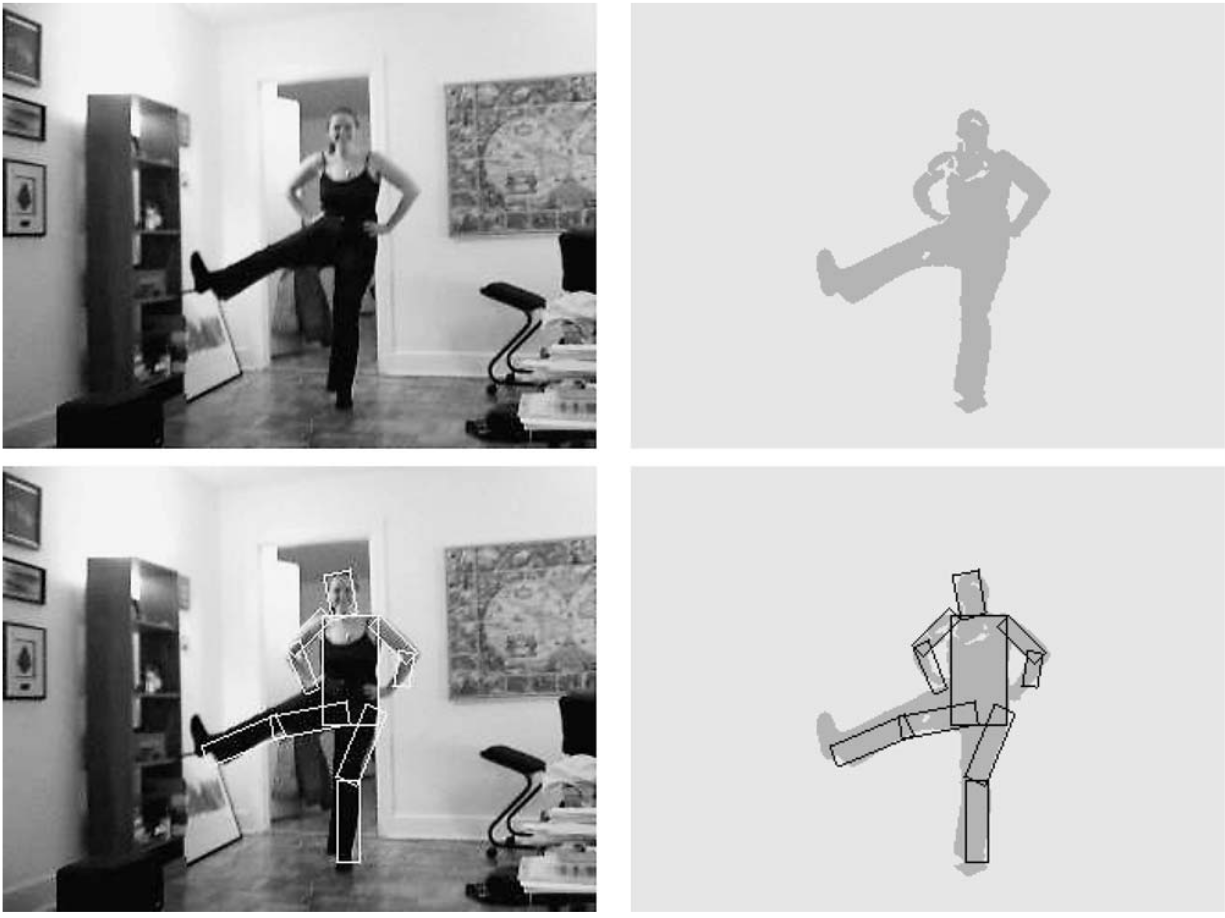
\includegraphics[width=0.8\textwidth]{felzenszwalb-overview.png}
    \caption{Overview of pose matching algorithm. \textbf{Upper left}: Original image. \textbf{Upper right}: binary image where foreground pixels (containing the human figure) are separated from the background. \textbf{Lower right}: One result from matching the limb rectangles to maximize the amount of foreground pixels covered. \textbf{Lower left}: Final result with estimated pose layered on top of original image. Image taken from \cite{felzenszwalb_pictorial_2005}.}
    \label{fig:felzenszwalb-overview}
\end{figure}

The authors model the human pose as a collection of $10$ different parts. 
Two parts per arm and leg as well as one torso and one head part \fref{fig:felzenszwalb-overview}.
Each part configuration $l_i = (x_i, y_i, s_i , \varphi_i)$ contains the $x$ and $y$ coordinate of the center of the rectangle representing the part.
In addition, $s_i \in [0,1]$ defines the length of the rectangle and $\varphi_i$ its rotation.
The width is fixed.

To model $p(I \mid l_i, \theta_i)$ they use the formula in \eref{eq:felz-unary} which utilizes $\theta_i = (q_1, q_2)$.
$q_1$ is the probability of pixel inside $l_i$ being a foreground pixel whereas $q_2$ is the probability of pixels closely around $l_i$ being foreground pixels.
The area around $l_1$ is referred to as $area_2$ whereas the area of $l_i$ is referred to as $area_1$.
$count_i$ referres to the number of foreground pixels in $area_i$ and $t$ is the total number of pixels in the image.

\begin{equation}
    \label{eq:felz-unary}
    \begin{split}
        p(I \mid l_i, (q_1, q_2)) = &q_1^{count_1} * (1 - q_1)^{(area_1 - count_1)} \\ 
        &* q_2^{count_2} * (1 - q_2)^{(area_2 - count_2)} \\ 
        &* 0.5^{(t - area_1 - area_2)}
    \end{split}
\end{equation}

Also, they smooth the distribution to prevent peaks by using the principle of annealing with a constant factor $T$ \eref{eq:smoothed}.
This is important because a distribution with strong peaks is more likely to return similar results when sampled from.
As discussed earlier, sampling is needed because of the approximation of the unary term the authors used and its problem with overlapping limbs.
A distribution with too strong peaks would not allow for sufficiently different pose samples.

$\theta_i$ is then estimated using mean values from annotated training data points while $T$ is set to $10$.

\begin{equation}
    \label{eq:smoothed}
    p(I \mid l_i, \theta_i) \propto p(I \mid l_i, \theta_i)^{\frac{1}{T}}
\end{equation}

\begin{figure}[htb!]
    \centering
    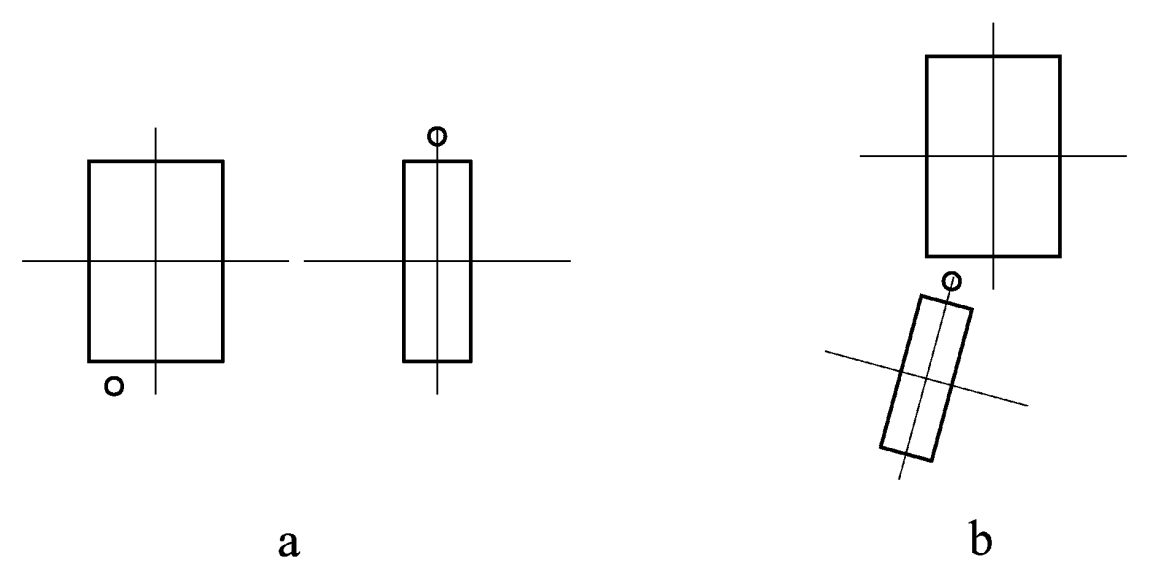
\includegraphics[width=0.8\textwidth]{limb-connection.png}
    \caption{Visualization of connecting limbs. \textbf{a}: Two limbs in their own coordinate system. The circles indicate connection joints. \textbf{b}: Possible, anatomically plausible connection. Image taken from \cite{felzenszwalb_pictorial_2005}.}
    \label{fig:limb-connection}
\end{figure}

Next, the authors model the prior $p(L \mid \theta)$.
Each spatial relation $p(l_i, l_j \mid \theta)$ between two parts is modelled in the following way:
First, each part is placed inside its own coordinate system with the origin being the center point of the part (see Figure \ref{fig:limb-connection}a).
The connection point (joint) between parts $i$ and $j$ is defined as $(x_{ij}, y_{ij})$ in the coordinate system of part $i$ and as $(x_{ji}, y_{ji})$ in the coordinate system of part $j$.
When transformed to the image coordinate system, these points should be as close together as possible (see Figure \ref{fig:limb-connection}b).
The authors express this using Gaussian distributions:

\begin{equation}
    \begin{split}
        N((\hat{x}_i - \hat{x}_j), 0, \sigma^2_x) \\
        N((\hat{y}_i - \hat{y}_j), 0, \sigma^2_y),       
    \end{split}
\end{equation}

where $\hat{x}_i$ and $\hat{y}_i$ are transformations of the joint position into the image coordinate system:

\begin{equation}
    \begin{bmatrix}
        \hat{x}_i \\ 
        \hat{y}_i
    \end{bmatrix}
    =
    \begin{bmatrix}
        x_i \\ 
        y_i
    \end{bmatrix}
    + s_i R_{\varphi_i}
    \begin{bmatrix}
        x_{ij} \\ 
        y_{ij}
    \end{bmatrix}.
\end{equation}

$\hat{x}_j$ and $\hat{y}_j$ are computed analogously.
$R_{\varphi_i}$ is a matrix which rotates around the origin for $\varphi_i$ radiants.
Additionaly, the authors define that the difference between $s_i$ and $s_j$ should be close to zero as well.
Again, this is modelled using a Gaussian distribution:

\begin{equation}
    N((s_i - s_j), 0, \sigma^2_s).
\end{equation}

Lastly, the authors specify that the difference between the two relative angles $\varphi_i$ and $\varphi_j$ be close to a parameter $\varphi_{ij}$.
They use a von Mises distribution, given by

\begin{equation}
    M(\theta, \mu, k) \propto \exp (k \cdot \cos (\theta - \mu)).
\end{equation}

A von Mises distribution can be thought of as a normal distribution around a circle, which is why the authors use it for periodic input like gradients.
Using $\mu = \varphi_{ij}$ they specify the constrained described earlier.
The parameter $k$ determines how strong the peak at $\varphi_{ij}$ should be or, in other words, how constrained the joints should be.

In summary, each spatial relation is expressed in the following way:

\begin{equation}
    \begin{split}
        p(l_i, l_j \mid \theta) 
        &= p(l_i, l_j \mid c_{ij}) \\
        &= N((\hat{x}_i - \hat{x}_j), 0, \sigma_x^2) \\
        &* N((\hat{y}_i - \hat{y}_j), 0, \sigma_y^2) \\
        &* N((s_i - s_j), 0, \sigma_s^2) \\
        &* M((\varphi_i - \varphi_j), \varphi_{ij}, k).
    \end{split}    
\end{equation}

The prior parameters $c_{ij}$ are then given by $c_{ij} = (x_{ij}, x_{ji}, y_{ij}, y_{ji}, \sigma_x, \sigma_y, \sigma_s, \varphi_{ij}, k)$ and are estimated using maximum likelihood estimation.

% ----- Short evaluation
The authors merely provide example images instead of a quantitative analysis.
This is most likely because of the lack of benchmark data sets available at the time.
They labeled $10$ images by hand and used these to estimate the parameters.
Then, for each of their unlabeld test images, they sampled $200$ poses and calculated the Chamfer distance, which measures the binary correlation.
The best pose with regards to the Chamfer distance is then returned.
Some example images can be seen in \fref{fig:pictoral-examples}

\begin{figure}[htb!]
    \centering
    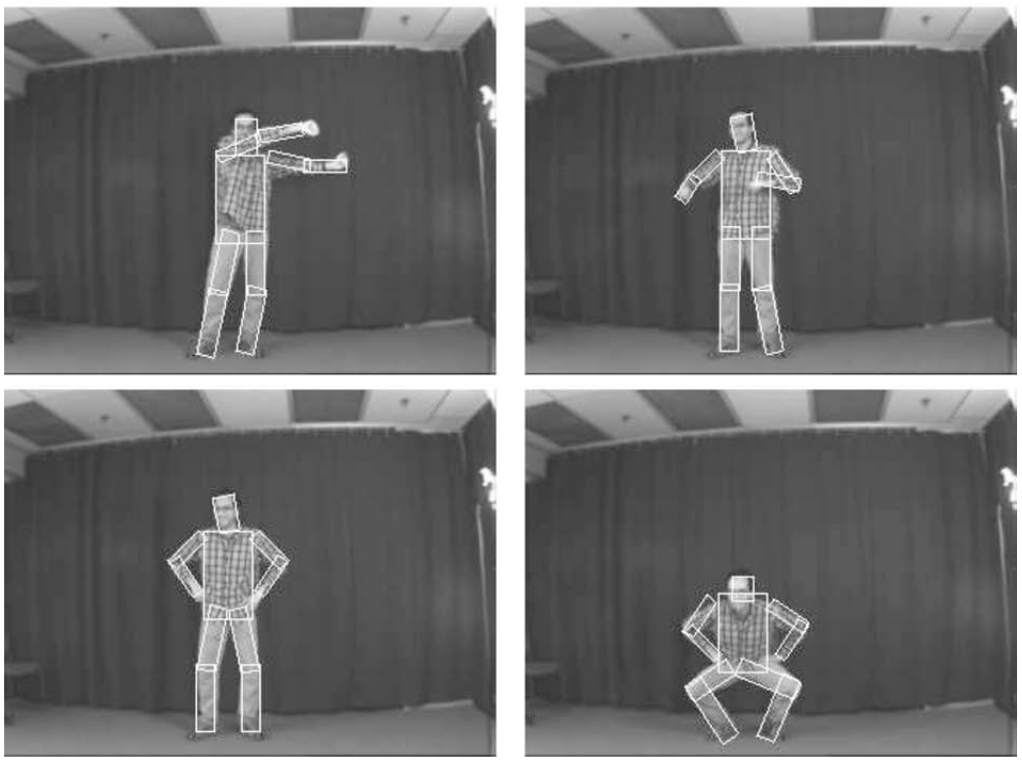
\includegraphics[width=0.8\textwidth]{pictoral-examples.png}
    \caption{Example of poses estimated by the statistical framework. Image taken from \cite{felzenszwalb_pictorial_2005}.}
    \label{fig:pictoral-examples}
\end{figure}

\subsubsection{Approaches for parts detection}
\label{sec:pose-andriluka}
% TODO: say that many different over the years (maybe cite some?) but here just one in-depth

In \cite{andriluka_pictorial_2009}, the authors propose a different appearance model $p(I \mid L, \theta)$, which is based on individual parts detectors.
\cite{felzenszwalb_pictorial_2005} used background separation to extract the silhouette of the subject from the background.
Then, the objective was to configure the parts in such way that the covered foreground area was maximized (see \eref{eq:felz-unary}).
This resulted in a large search space since all different rotations and scalings for each part need to be placed inside the foreground area in order to evaluate the overall fit.
The authors in \cite{andriluka_pictorial_2009} limit the search space by using a detected \textit{parts evidence map} $d_i$ for each part $i$.
An example evidence map can be seen in \fref{fig:parts-evidence}.
These evidence maps are the result of individual parts detectors trained on annotated images such as presented in \fref{fig:parts-annot}.
To compute the evidence map, parts detectors are trained using annotated training data.

\begin{figure}
    \centering
    \subfloat[Parts-annotated example image.\label{fig:parts-annot}]{%
        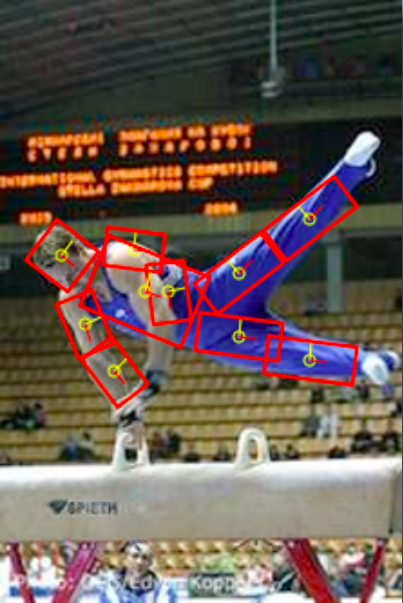
\includegraphics[height=150px]{poseparts.png}
    }
    \hspace{20px}
    \subfloat[Part evidence map for part \textit{head}. Notice the peak (in red) where the head is in the left image.\label{fig:parts-evidence}]{%
    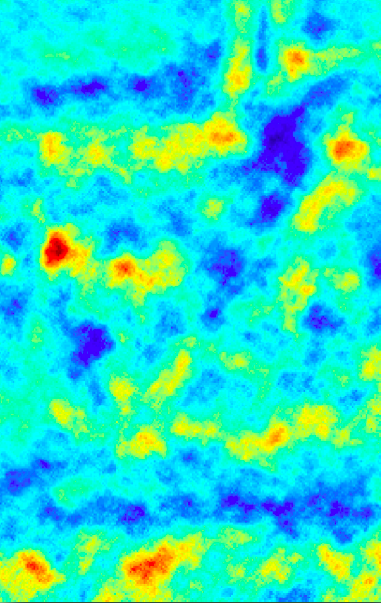
\includegraphics[height=150px]{partevidence.png}
}
    \caption{Images taken from corresponding talk to \cite{andriluka_pictorial_2009}.}
\end{figure}

% Descriptors
The authors compute dense \textit{shape context descriptors} \cite{belongie_shape_2002} for each training image.
This local descriptor takes gradients of edge pixels into account and discretizes them into bins in a log-polar histogram.
The authors chose $12$ bins for the location where the gradients are put inside $8$ bins, resulting in a $96$ dimensional descriptor for each sampled point.
Descriptors with a center point inside a part bounding box given by the annotation are then concatenated and used as positive training examples to train the parts detectors.

% Detectors
For detectors, the authors use the concept of \textit{boosting} where the decisions of many weak classifiers are combined into a strong classifier \cite{freund_short_1999}.
Specifically, the authors use the \textit{AdaBoost} algorithm proposed by \cite{freund_decision-theoretic_1997}.
Each weak detector takes a bin from the feature vector and compares it to a threshold.
The sign of the result is then used as the output of the weak detector following

\begin{equation}
    h_t(\bm{x}) = sign(\xi_t (\bm{x}_{n(t)} - \varphi_t )),
\end{equation}

where $\bm{x}$ is the feature vector, $\xi_t \in \{-1, 1\}$ and $n(t)$ is the index of the bin, which is used to compare to $\varphi_t$.
The authors do not, however, specify how to set $\xi_t$ or which threshold $\varphi_t$ was used.

Combining $t$ weak detectors by summing over the weighted outputs, the complete part detector for part $i$ is given by 

\begin{equation}
    H_i(\bm{x}) = sign\left(\sum_t a_{i,t} h_t(\bm{x})\right)
\end{equation}

According to the authors, $a_{i,t}$ are weights learned by each weak detector.
To fit the parts detectors into the Pictoral Structure Framework, the authors compute a pseudo-probability based on the part detectors:

\begin{equation}
    p(d_i \mid l_i) = max \left(\frac{\sum_t a_{i,t} h_t(\bm{x}(l_i))}{\sum_t a_{i,j}}, \epsilon_0 \right).
\end{equation}

$\bm{x}(l_i)$ is the feature vector for part $l_i$ whereas $\epsilon_0$ is set to $10^{-4}$.
The authors claim that this pseudo-probability achieves good results in practice.

% Appearance model Pictoral Structure Framework
Lastly, the authors make two assumptions in order to embed the parts detectors into the Pictoral Structute Framework.
First, different part evidence maps $d_i$ are independent from each other given $L$.
Second, $d_i$ only depends on $l_i$ on not on other parts configurations.
This leads to the following likelihood

\begin{equation}
    p(I \mid L, \theta) = p(D \mid L) = \prod_{i=0}^N p(d_i \mid l_i),
\end{equation}

where $N$ is the number of parts to detect in the given image.

% Evaluation
The authors use two datasets to evaluate their model.
The \textit{Buffy} dataset provides annotated upper-body poses from $3$ episodes of the TV series \textit{Buffy The Vampire Slayer} \cite{ferrari_progressive_2008}.
Also, for evaluating full-body poses, they used the \textit{Iterative Image Parsing} dataset providid by \cite{ramanan_learning_2007}

As an evaluation metrc, the authors use \textit{Percentage of Correct Parts (PCP)}, proposed by \cite{ferrari_progressive_2008}.
For each annotated body part, PCP is calculated by first computing the length of the ground truth body part $l_{gt}$.
Then, a threshold value $t_{gt} = 0.5 \cdot l_{gt}$ is defined as half the length of the segment.
If both endpoints of a prediction fall within $t_{gt}$ radius of their ground truth annotation the part is considered detected.

First, they compare their upper-body model to \cite{ferrari_progressive_2008}.
In contrast to \cite{ferrari_progressive_2008}, however, the authors also compute PCP for each part, whereas \cite{ferrari_progressive_2008} only provide the overall accuracy of $57.9\%$.
Using the pose dataset of \cite{ramanan_learning_2007} for training the pose priors and part detectors, the authors achieve an overall accuracy of $71.3\%$.
They notice that, while torso, head and upper arm accuracy is fairly high (from $78\%$ for upper arm to $95.9\%$ for head), forearm accuracy ($40\%$) was significantly lower.
They argue that is is due to the challenging nature of the dataset.
Also, forearm parts are smaller, making it more difficult for parts to be considered correct.
The authors also tried exclusively using frames from the Buffy dataset, which were not used for testing, to learn the pose priors.
This lead to a slight increase in accuracy ($73.5\%$) in comparison to generic priors, mainly by increasing the forearm accuracy scores.
This illustrates that generic pose priors can achieve comparable results to domain-specific priors.

For evaluating full body pose, the authors compared their results to the results presented by \cite{ramanan_learning_2007}, the authors of the dataset.
Overall, they achieve an overall accuracy of $55.2\%$, which is significantly higher than the $27.2\%$ achieved by \cite{ramanan_learning_2007}.
The authors argue that this large improvement is due to their strong part detector.
This is illustrated by the accuracy achieved on the head part.
The accuracy of the authors is higher than \cite{ramanan_learning_2007}, even when not using the pose prior information and just using the part detector.


% TODO: A little bit about the tree prior (didnt deviate too much, but lets find a little detail thats different)


\subsubsection{Articulated pose estimation with flexible mixture-of-parts}

Another approach building on the Pictoral Structure Framework was proposed by \cite{yang_articulated_2011}.

The proposed model differs from the Framework by using parts which are not rotated or forshortened.
To gain more flexibility, each part $i$ has a type $t_i$, which can encode arbitrary information, since the model the authors propose is general.
One possibility, which is also what the authors used in their experiments, is to let the types correspond to different orientations.
For example, two types for the part \textit{head} could be \textit{upright} or \textit{tilted to the left}.
In addition, in this model, it is possible to constraint two adjacent parts' types as will be seen later.

% General overview over differences
First, the authors change the definition of a part $i$ and its parametrization $l_i$ from the one presented in \cite{felzenszwalb_pictorial_2005}.
A part is defined as a joint instead of a limb because the data sets used annotated joint positions as opposed to parts positions.
Thus, the parametrization changes to $l_i = (x_i, y_i)$ since no rotation and forshortening occurs.

% Learning
%% Generate annotation
The data sets the authors used do not provide annotations for type labels, which is why these were computed beforehand using the following steps.
First, the authors define a graph where the vertices correspond to joints.
The edges of the graph are defined in a way that model a human skeleton.
See \fref{fig:yang-tree} for an example graph.

\begin{figure}[htb!]
    \centering
    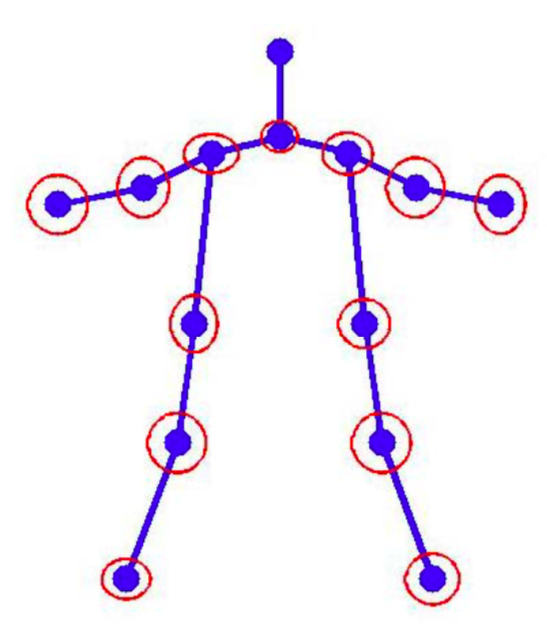
\includegraphics[width=0.35\textwidth]{yang-tree.png}
    \caption{Visualisation of the graph resulting from connecting the joint positions, which form the vertices, together into a human skeleton. Image taken from \cite{yang_articulated_2011}.}
    \label{fig:yang-tree}
\end{figure}

Second, the orientation of a part $i$ is considered relative to its parent part $j$.
For instance, consider the relative position of the part corresponding to \textit{neck} to its parent part \textit{head}.
Necks tend to be below heads (for upright people).
The authors use all relative positions found by iterating the dataset and cluster the relative positions into $T=4$ clusters.
The cluster that the part $i$ is put in then defines the type label $t_i$.
See \fref{fig:yang-clustering} for an example.
This then results in a fully annotated data set with location information $l_i$ as well as type $t_i$ for each part $i$.

\begin{figure}[htb!]
    \centering
    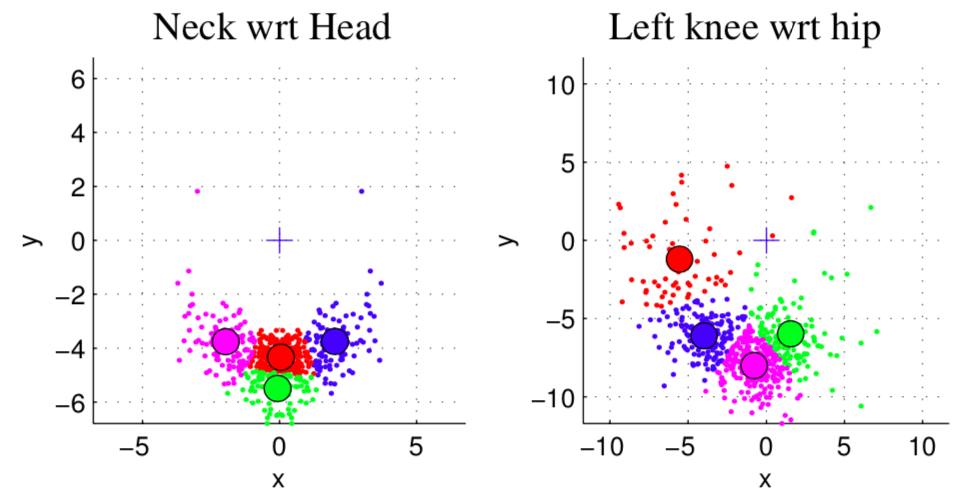
\includegraphics[width=0.65\textwidth]{yang-clustering.png}
    \caption{The relative positions of \textit{neck} with regard to     its parent \textit{head} (\textbf{left}) and \textit{left knee} with regard to \textit{hip} (\textbf{right}). The origin marks the location of the parent. Notice that the neck is generally placed below the head (since most images contain upright people) while the left knee is mostly placed left of the hip. Each color indicates a cluster and a thus a corresponding type label. Image taken from \cite{yang_articulated_2011}.}
    \label{fig:yang-clustering}
\end{figure}

Instead of using one \textit{template} for each limb, the authors propose to use many small templates per limb.
Each template can be of a specific type $t_i$, which can encode semantic features, e.g., open versus closed hand, or orientational information.

%% Score function
The authors provide the following score function to evaluate a predicted pose:

\begin{equation}
    \label{eq:yang-score}
    \begin{split}
        S(I, l, t) 
        &= \sum_{i \in V} b_i^{t_i} + w_i^{t_i} \cdot \phi(I, l_i) \\
        &+ \sum_{(i,j) \in E} b_{ij}^{t_i, t_j} + w_{ij}^{t_i, t_j} \cdot \psi(l_i - l_j)
    \end{split}
\end{equation}

In \eref{eq:yang-score}, $I$ refers to the image that is evaluated.
$l = (l_1, \cdots, l_k)$ is the configuration containing all part positions while $t = (t_1, \dots, t_k)$ corresponds to the types of parts.
$\phi(I, l_i)$ is a HOG feature vector \cite{dalal_histograms_2005} computed around the part position $l_i$.
$\psi(l_i - l_j) = [(x_i - x_j), (x_i - x_j)^2, (y_i - y_j), (y_i - y_j)^2]^T$ encodes the relative location of part $l_i$ to $l_j$.

$w_i^{t_i}$, $w_{ij}^{t_i, t_j}$ as well as $b_i^{t_i}$ and $b_{ij}^{t_i, t_j}$ are parameters estimated from annotated training data, which encode learned relationships between parts as well as type assignments for each part.
During training, a supervised approach is used where the score for an annotated training image is maximized while utilizing regularisation on the models parameters $\beta = (\bm{w}, \bm{w})$.

% Evaluation
To evaluate their model, the authors use Percentage of Correct Parts (PCP) \cite{ferrari_progressive_2008} to be able to compare it to earlier work.
In addition, they define two new metrics, \textit{PCK} (Probability of Correct Keypoints) as well as \textit{APK} (Average Precision of Keypoints).

%% TODO: Finish evaluation
In PCP, a limb is defined as being detected correctly if 

Authors propose PCK
Authors propose APK

\begin{figure}[htb!]
    \centering
    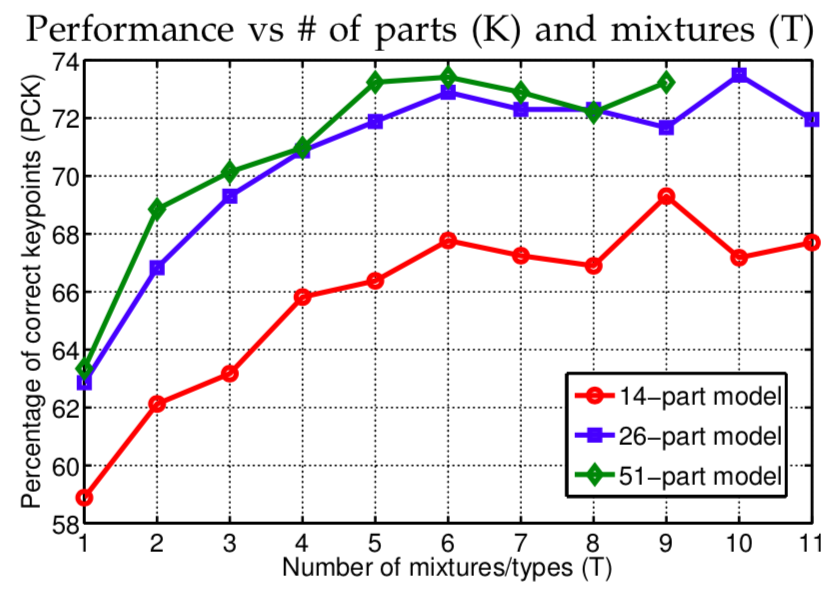
\includegraphics[width=0.5\textwidth]{yang-results-chart.png}
    \caption{The authors find that the higher the number of mixtures ($T$) the higher the accuracy. This is also true, to an extend, with number of parts to detect ($K$). The authors suggest a $26$ part, $6$ mixture model for a good trade-off between accuracy and performance. Image taken from \cite{yang_articulated_2011}.}
    \label{fig:yang-results-chart}
\end{figure}

\subsection{Deep Learning Methods}

\subsubsection{DeepPose}
% Introduction
One of the first approaches for pose estimation using deep convolutional neural networks was proposed by \cite{toshev_deeppose:_2014}.
They achieved state-of-the-art results on two benchmark datasets using a neural network architecture based on the ImageNet network \cite{krizhevsky_imagenet_2012}.
In contrast to the pictoral structure framework discussed earlier, the approach was to regress the image coordinates directly without specific constrains on how the joints are allowed to be connected.

% Architecture
The authors define their network in terms of multiple connected \textit{stages}.
Each \textit{stage} is comprised of the neural network architecture proposed by \cite{krizhevsky_imagenet_2012}.
The used architecture is provied in Table \ref{tab:deeppose-architecture}.
The only change the authors made was to use the output of the last fully connected layer to regress the joint coordinates as opposed to the softmax activation present in \cite{krizhevsky_imagenet_2012}.
This means that, assuming $k$ joints, the output of a stage is of size $2 * k$.
Stage $s_0$ is trained using the full images of size $220 x 220$ as its input.
Once the first stage is trained until convergence, the authors use the output coordinates to crop sub images around the initially predicted joint coordinates.
By feeding these subimages into another stage $s_1$ they argue that the predictions get more precise because local context becomes more important.
This cascading approach is then repeated with the next stages.
In the end, they use $3$ stages $S = (s_0, s_1, s_2)$ after evaluating different numbers of stages on a held-out training set.

\begin{table}[]
    \begin{tabular}{|l|l|l|l|l|}
    \hline
    \textbf{nr.} & \textbf{layer type} & \textbf{filter size} & \textbf{nr. of filters / neurons} & \textbf{stride} \\ \hline
    1 & convolutional & 11 x 11 x 3 & 96 & 4 \\
    2 & local response normalization &  &  &  \\
    3 & pooling & 3 x 3 &  & 2 \\ \hline
    4 & convolutional & 5 x 5 x 48 & 256 & 1 \\
    5 & local response normalization &  &  &  \\ 
    6 & pooling & 3 x 3 &  & 2 \\ \hline
    7 & convolutional & 3 x 3 x 256 & 384 & 1 \\
    8 & convolutional & 3 x 3 x 192 & 384 & 1 \\
    9 & convolutional & 3 x 3 x 192 & 256 & 1 \\ \hline
    10 & fully connected &  & 4096 &  \\
    11 & fully connected &  & 4096 &  \\ \hline
    12 & fully connected &  & 2k &  \\ \hline
    \end{tabular}
    \caption{One \textit{stage} of the DeepPose network. Architecture based on \cite{krizhevsky_imagenet_2012}.}
    \label{tab:deeppose-architecture}
\end{table}

% Evaluation
\begin{figure}[htb!]
    \centering
    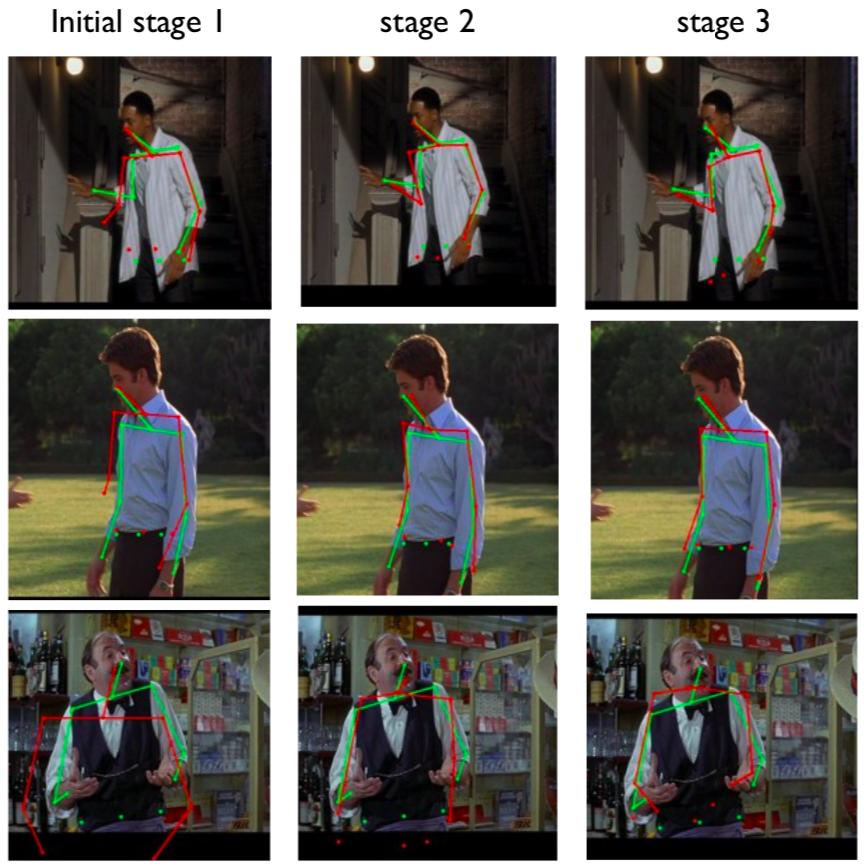
\includegraphics[width=0.5\textwidth]{deeppose-qualitative.png}
    \caption{Qualitative evaluation of the cascading architecture. Ground truth joints are shown in green while predicted poses are shown in red. Notice how the pose gets more accurate with consecutive stages. Also, notice that the biggest improvement can be seen after stage $1$. The authors argue that this is due to the fact that, with an increase in stages, the subimage gets smaller and smaller and thus harder to estimate the pose. Image taken from \cite{toshev_deeppose:_2014}.}
    \label{fig:deeppose-qualitative}
\end{figure}

% TODO: Move dataset / metric explanation if happening before
After training their network, the authors evaluate the final model on two datasets, FLIC \cite{sapp_modec:_2013} and LSP \cite{johnson_clustered_2010}.
Frames Labled In Cinema (FLIC) is a dataset which contains $5000$ images of Hollywoord movie scenes where $10$ upper body joint positions are labeled for the subject of the scene.
Leeds Sports Pose (LSP) is a dataset of $2000$ annotated images of subjects in a sport context.
LSP contains $14$ different joint positions of the entire body.

The authors use two different metrics to evaluate their model, PCP and PDJ.
The authors take the ground truth coordinates of the joints on the end of each limb to calculate the limb length for PCP.

PCP has the disadvantage that short limbs get penalized more than big limbs.
To overcome this shortcomming, the authors define a new evaluation metric called Percent of Detected Joints (PDJ).
With this metric, a joint is considered detected correctly if the distance between the predicted joint position and the ground truth $d_p$ is smaller than a fraction of the torsos diameter $d_t$.
This fraction is set to be $0.5$, meaning a joint is considered detected if $0 <= d_p <= 0.5 \cdot d_t$.
This metric is similar to PCK in that it compares the distance between two joints to a subject-specific value like torso diameter or subject bounding box, effectively normalizing the result.

The authors provide three examples which illustrate the importance of the cascading architecture.
These examples can be seen in \fref{fig:deeppose-qualitative}.
They argue that stage $s_1$ has the biggest effect on the accuracy of the joints since further stages use smaller and smaller subimages for regression and thus use a smaller context.

\subsubsection{Stacked Hourglass}

% Introduction
Building on \cite{toshev_deeppose:_2014}, \cite{newell_stacked_2016} proposed the \textit{Stacked hourglass network}.
In comparison to \cite{toshev_deeppose:_2014}, they do not regress the joint coordinates directly using fully-connected layers but use a fully convolutional architecture to compute \textit{heatmaps}.
These heatmaps are very similar to the part evidence maps discussed in Chapter \ref{sec:pose-andriluka}.
However, the heatmaps indicate the probability of a certain joint to be present instead of a part.

Similar to \cite{toshev_deeppose:_2014}, the authors use a stacked architecture, where predictions get refined iteratively.
They do, however, do not crop the input down with each iterative step but keep the whole image in every step.

\begin{figure}[htb!]
    \centering
    \includegraphics[width=0.8\textwidth]{stackedhourglass.png}
    \caption{Schematic visualization of the stacked hourglass network. Notice the hourglass-shaped symmetric submodels connected together. Image taken from \cite{newell_stacked_2016}. }
    \label{fig:stacked-hg-architecture}
\end{figure}

% Architecture
The building blocks of the stacked hourglass archtitecture are so-called \textit{hourglass modules}.
See \fref{fig:single-hourglass} for a visualization of a single hourglass module.
The idea is to process the input of the module at different scales and then combine features from different scales using \textit{skip-connections}.

\begin{figure}[htb!]
    \centering
    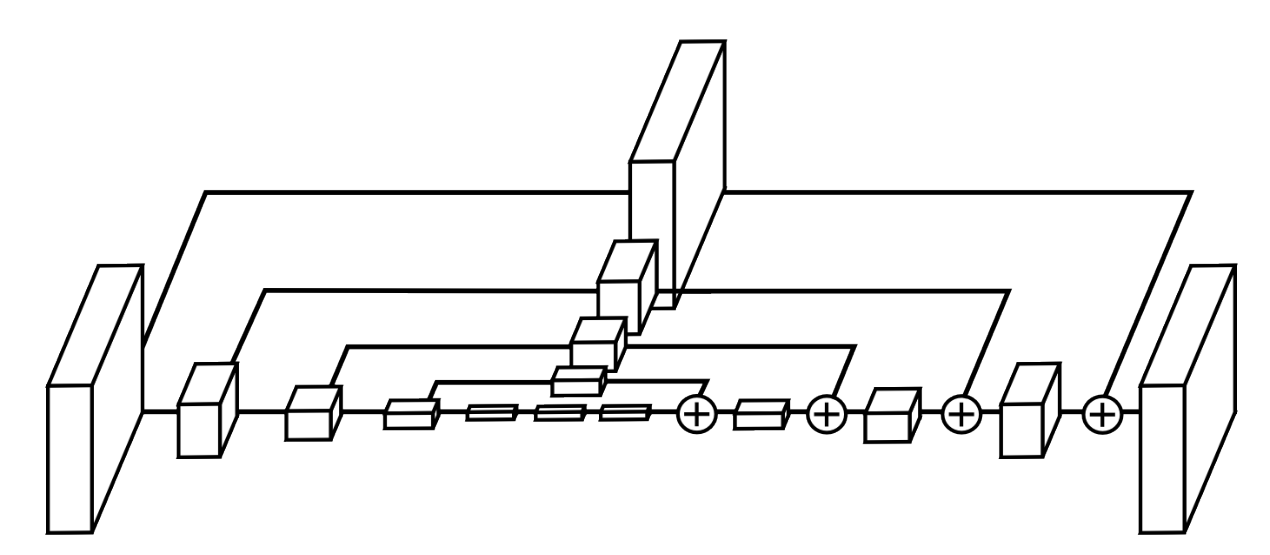
\includegraphics[width=0.6\textwidth]{single-hourglass.png}
    \caption{Visualization of a single hourglass module. Each block is a residual module, consisting of multiple convolutional layers with skip-connections. Notice how the skip-connections combine features at different scale levels. Image taken from \cite{newell_stacked_2016}. }
    \label{fig:single-hourglass}
\end{figure}

A skip-connection is a path in the network, which branches of at a certain point and gets combined with the original path again further down the network.
For example, consider a neural network with three convolutional layers.
A skip-connection could branch of before the first convolutional layer, apply some processing in forms of additional convolutional layers, and get added back into the original path after the second convolutional layer, thus effectively \textit{skipping} the processing of the first and second convolutional layers.
Thus, earlier features (in terms of network depth) can be reintroduced at a later stage.
One common use-case for skip-connections, which the authors used, is to reintroduce lower level features and add them to higher level features.
This way, tasks like pose estimation can incorporate global, high level features like body shape with low level, local features like faces.

Skip-connections get used in \textit{residual blocks} \cite{he_deep_2016}, which are used for more efficient learning in deep networks.
Consider two connected convolutional layer with input $x$.
Let $f(x)$ be the output of the second convolutional layer.
Residual models model $f(x) + x$ because they use the skip-connection to add the input back to the output.
The authors of \cite{he_deep_2016} argue that this allows for deeper neural network architectures because it is easier to fit identity mappings.
They evaluated deep neural networks and found that the error does not only not decrease for very deep networks but starts increasing.
The authors argue that this would not happen if the layers would learn identity functions because then the error would just stagnate.
In addition, because residual blocks allow for very deep architectures, they achieved substantially better results in comparison to identical architectures without residual blocks.

An example of a residual blocks used in the stacked hourglass network can be seen in \fref{fig:hg-residual}.
In fact, all blocks shown in \fref{fig:single-hourglass} are residual blocks.

\begin{figure}[htb!]
    \centering
    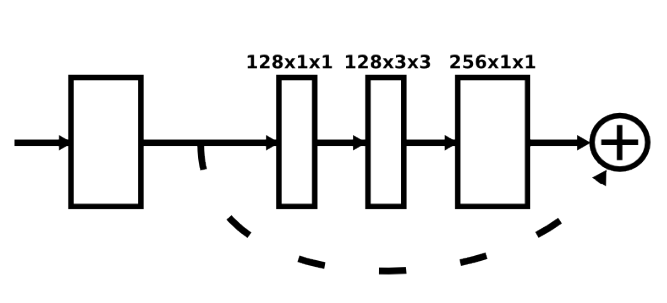
\includegraphics[width=0.4\textwidth]{residualmodule.png}
    \caption{A residual module \cite{he_deep_2016}, as used in the stacked hourglass network. The module is made up of a batch normalization layer (left) and three convolutional layers, each utilizing the ReLU activation function. The dotted line visualizes the skip-connection. Image taken from \cite{newell_stacked_2016}. }
    \label{fig:hg-residual}
\end{figure}

Each hourglass module is a network with a symmetrical architecture.
For each downsampling step with a pooling layer there exists a corresponding upsampling step using \textit{nearest-neighbour upsampling}.
Consequently, the input and output dimensions of the hourglass module are identical, allowing multiple modules to be applied one after the other.

The input to the module is scaled down using pooling layers, until it reaches a resolution of $4x4$ pixels.
Before each pooling layer, a skip-connection is utilized to branch off the current feature maps.
They get feed through another residual block and combined back later.

At each resolution level, features are extracted using a residual module.
Once image is scaled down to $4x4$ pixels, upsampling is utilized until the image is back to its original size.
Again, residual blocks are used to extract features at the different levels of resolution.
Also, after the feature extraction, the processed skip-connections from earlier get added onto the extracted features, effectively combining features from two different image scales, because they get combined before upsampling happens.

The authors use another skip-connection between the input and output of the module.
This means that the input to each module, which is the output of the previous module, is added onto its output.
The authors argue that this allows the network to refine its prediction with each hourglass module since the high level features, which are the outputs of each module, get processed by consecutive hourglass modules again, creating higher order spatial relationships.
They qualitatively observe that errors made by early modules can be corrected by later modules.
Also, they evaluated the difference between $2, 4$ and $8$ stacked hourglasses, which will be referred to as $s_2, s_4$ and $s_8$.
For a better comparability, they altered the hourglass archictecture for the $s_2$ and $s_4$ to keep the number of trainable parameters the same between architectures.
For each residual block in each hourglass in $s_2$ the authors substituted $4$ residual blocks, effectively quadrupeling the number of residual blocks.
Analogously, they doubled the amount of residual blocks for $s_4$.
When training $s_2, s_4$ and $s_8$, they found validation accuracies of $87.4\%$, $87.8\%$ and $88.1\%$ respectively, suggesting that the stacked architecture does contribute to higher overall accuracies.
In the final architecture, the authors use $8$ hourglass modules.

While training, the output of each hourglass module is not only feed into the next module, but also processed into a \textit{heatmap} using a $1x1$ convolutional layer.
Using this heatmap, a loss is computed after each hourglass module, which is then propagated back.
The authors refer to this process as \textit{intermediate supervision} and argue that it increases the accuracy of the final prediction because the network needs to develop a high-level of understanding very early.
In their quantitative analysis, they showed an increase in validation accuracy of around $3$ percent when utilizing intermediate supervision. 

% Evalutation
%% Meassurements and Datasets
For evaluating the stacked archictecture, the authors used the \textit{FLIC} and \textit{MPII Human Pose}\cite{andriluka_2d_2014} data sets.

MPII Human Pose is a benchmark, which consists of $40,000$ annotated images of people.
These images are also often referred to as \textit{in-the-wild} images since they were downloaded from YouTube videos and are thus representative of every day activaties and situations.
In addition, since most YouTube videos are uploaded by private individuals, the image quality varies, making the benchmark more realisitic.

The authors use \textit{PCKh} as their metric, which is identical to \textit{PCK} but instead of using the person bounding box the head bounding box is used for normalization.
For \textit{FLIC}, they defined a joint to be detected if the distance between the ground truth location and the predicted location is within $20\%$ of the head size.
With \textit{MPII Human Pose}, the threshold was reduced to $50\%$ in accordance to the previous works they compared against.


\begin{itemize}
    \item Convolutional Pose Machine \cite{wei_convolutional_2016}
    %\item Thin-Slicing Network \cite{song_thin-slicing_2017}
\end{itemize}

\section{Video-based Human Action Recognition}

Different approaches.
Some: frame-by-frame and just concatenate.
Other: Use temporal information.
Here: Only those who use temporal information.

\subsection{Shallow Methods}
\begin{itemize}
    \item Learning Realisitic Human Actions from Movies \cite{laptev_learning_2008}
\end{itemize}

\subsection{Deep Methods}
\begin{itemize}
    \item MiCT \cite{zhou_mict:_2018}
\end{itemize}